\documentclass[11pt]{article}
\title {MRes Proposal: Prioritising fish evolutionary history for conservation action}
\author{Oenone Scott}
\date{2 Dec 2019}
\usepackage[margin=2cm]{geometry}
\usepackage{graphicx}
\usepackage[]{lineno}
\usepackage[backend=biber,style=authoryear,bibencoding=utf8]{biblatex}


% bibliography secion %

\addbibresource{MResProposal.bib}

\begin{document}

\begin{titlepage}


	\centering % this centers everything on the page
		
	%\vspace  % Whitespace at the top of the page 
	
	
	% --------------------------
	%% TITLE
	
	\vspace*{5\baselineskip}
	
	\rule{\textwidth}{1.6pt}\vspace*{-\baselineskip}\vspace*{2pt} % Thick horizontal rule
	\rule{\textwidth}{0.4pt} % Thin horizontal rule
	
	\vspace{0.75\baselineskip} % Whitespace above the title
	
	{\LARGE PRIOTITISING FISH EVOLUTIONARY \\ HISTORY  \\ FOR CONSERVATION ACTION\\} 
	
	\vspace{0.75\baselineskip} % Whitespace below the title
	
	\rule{\textwidth}{0.4pt}\vspace*{-\baselineskip}\vspace{3.2pt} 
	\rule{\textwidth}{1.6pt} 
	
	\vspace{2\baselineskip} 
	
	% ---------------------------------
	%% SUPERVISORS & CONTACT EMAIL
	
	Supervisors: \\
		Dr. James Rosindell, Imperial College London \\
		Rikki Gumbs, Zoological Soceity of London	

		
	\vspace{1.5 \baselineskip} % Whitespace between text
	
	Contact: \\
	ojs19@imperial.ac.uk
	


\end{titlepage}

\linenumbers

	\section{Key Words}
	\begin{itemize}
	
	\item Conservation
	\item Genetics
	\item Phylogenetic diversity
	\item Computational
	\item Marine biology
	\item Quantitative
	\end{itemize}
	
	\section{Introduction}
	\noindent
	
We are currently undergoing the 'sixth mass extinction', which is widely attributed to be caused by human action \autocite{Barnosky2011a}. If we wish to preserve the biodiversity of the planet, there is an urgent need to act swiftly to preserve what is left \autocite{Barnosky2011a}. There are limited resources available for conservation work, and therefore it would be beneficial to have a way to 'rank' or prioritise organisms that require the most protection. \\

The EDGE programme is a programme designed for this purpose. The analysis scores species according to how Evolutionary Distinct and Globally Endangered they are \autocite{Isaac2007a}. These EDGE scores are used to inform conservation action and policy across the world \autocite{Isaac2007a}. \\

EDGE lists have been created for many clades of organisms, but nothing has yet been done for ray-finned fish. This project aims to start the process for the EDGE analysis of ray-finned fish. 

	\section{Methods}
	\noindent
	
To determine which clade within the ray-finned fish group should be selected for EDGE analysis in this project, we will run workshops with the marine experts at ZSL. This project will not be aiming to create an EDGE list for every ray-finned fish species, as there are approximately 31,000 species. \\

To perform the EDGE analysis we will use two data sources. The endangered status of the species will be taken from IUCN Red List extinction risk data, where available \cite{}. The phylogenetic trees will be sourced from publicly available data, which is available from http://fishtreeoflife.org \autocite{Rabosky2018}. The evolutionary-distinctness of the species can be calculated in a number of ways, and this project will drawn from the methodology developed by \cite{Gumbs2018}, \cite{Faith2008}, and \cite{Steel2007}. \\


The majority of the computational work in this project will be performed in R, as there are a number of packages developed specifically for this type of work. \\ 

Once EDGE analysis has been performed on the chosen clade(s), this project will work further with the marine team at ZSL and do desk research to discover if there are any conservation efforts underway for any of the species in the clade, and produce an analysis of any action that is being taken. 

	
\begin{figure}[h!]
	
	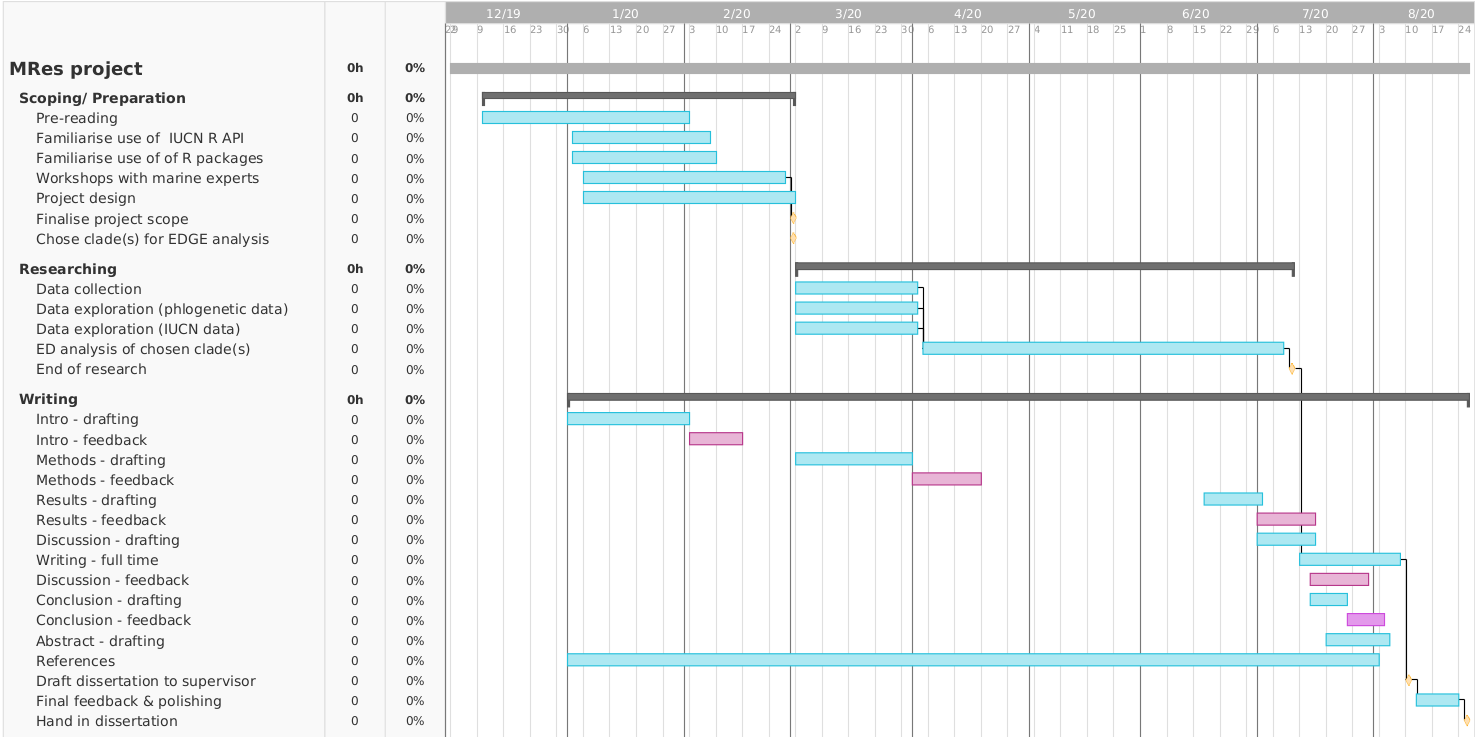
\includegraphics[width = \linewidth]{Images/Gantt_Image.png}
	\caption{	Gantt Chart}
	\label{MRes Gantt}
	
\end{figure}

\newpage

	
	\section{Anticipated outcomes}
	\noindent
	
	The anticipated outcomes of this project are:
	\begin{itemize}
	 \item An EDGE list for a clade/clades within the group of ray-finned fish
	 \item An updated methodology that could be applied to the other clades within this group. 
	 \item An analysis of the current conservation initiatives that apply to the species within the EDGE list. 
	\end{itemize}
	
	
	\section{Budget}
	\noindent
	
		The majority of the budget for this project will go towards travel between ZSL and Silwood, with the remained for some computing hardware. 
		
	\begin{itemize}
		\item Equipment: hard drive: £40 \\ This will be used to back-up all of the work. Online back-up with also be used to store specific work (e.g. github for code). 
		\item Equipment: projector: £40 \\ Projectors can be used to help de-bug code by projecting it onto whiteboards and walking through step by step. As this project will be very computationally intense, this tool is likely to be used very frequently. 
		\item Travel: Silwood - London: \pounds12 * 30 trips = \pounds360
		\item \textbf{Total: \pounds440}
	\end{itemize}
	
	
	\newpage
	  

	\vspace*{1\baselineskip}
	\printbibliography 


\newpage

	\section{Supervisor approval}
	\noindent
	
	I have seen and approved the proposal and the budget. \\ \\ 
	
	
	Supervisor name: Dr. James Rosindell \\ \\ 
	
	 
	
	Supervisor signature: 
	\begin{figure}[h!]
		
		
\includegraphics{Images/jrsignature.png}


		
	\end{figure}


\end{document}